\uuid{WlB5}
\exo7id{4994}
\titre{exo7 4994}
\auteur{quercia}
\organisation{exo7}
\datecreate{2010-03-17}
\isIndication{false}
\isCorrection{true}
\chapitre{Courbes planes}
\sousChapitre{Courbes définies par une condition}
\module{Géométrie}
\niveau{L2}
\difficulte{}

\contenu{
\texte{
Soit $\mathcal{C}$ une courbe du plan. A un point $M$ un point de $\mathcal{C}$, on associe les
points $H$, $T$ et $N$ selon le dessin :
$$
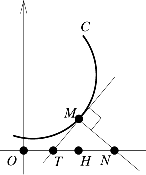
\includegraphics[height=3cm]{../images/pdf/WlB5-1.pdf}
$$

Déterminer les courbes d'équation $y = f(x)$ vérifiant la condition suivante :
}
\begin{enumerate}
    \item \question{$\overline{HT} ={}$cste.}
\reponse{$y = ae^{bx}$.}
    \item \question{$\overline{HN} ={}$cste.}
\reponse{$y = \pm\sqrt{ax+b}$.}
    \item \question{$MN = {}$cste.}
\reponse{$(a-x)^2 + y^2 = b^2$.}
    \item \question{$MT = {}$cste.}
\reponse{$x = a\left(\ln\left|\tan\frac t2\right| + \cos t\right) + b,\quad
              y = a\sin t$.}
    \item \question{$AN=MN$ où $A$ est le point de coordonnées $(0,a)$.}
\reponse{$y^2 = \frac{x^2}2 + a^2\ln|x| + b$.}
\end{enumerate}
}
